\documentclass[UTF8]{ctexart}
\usepackage{geometry, CJKutf8}
\geometry{margin=1.5cm, vmargin={0pt,1cm}}
\setlength{\topmargin}{-1cm}
\setlength{\paperheight}{29.7cm}
\setlength{\textheight}{25.3cm}

% useful packages.
\usepackage{amsfonts}
\usepackage{amsmath}
\usepackage{amssymb}
\usepackage{amsthm}
\usepackage{enumerate}
\usepackage{graphicx}
\usepackage{multicol}
\usepackage{fancyhdr}
\usepackage{layout}
\usepackage{listings}
\usepackage{float, caption}

\lstset{
    basicstyle=\ttfamily, basewidth=0.5em
}

% some common command
\newcommand{\dif}{\mathrm{d}}
\newcommand{\avg}[1]{\left\langle #1 \right\rangle}
\newcommand{\difFrac}[2]{\frac{\dif #1}{\dif #2}}
\newcommand{\pdfFrac}[2]{\frac{\partial #1}{\partial #2}}
\newcommand{\OFL}{\mathrm{OFL}}
\newcommand{\UFL}{\mathrm{UFL}}
\newcommand{\fl}{\mathrm{fl}}
\newcommand{\op}{\odot}
\newcommand{\Eabs}{E_{\mathrm{abs}}}
\newcommand{\Erel}{E_{\mathrm{rel}}}

\begin{document}

\pagestyle{fancy}
\fancyhead{}
\lhead{韩箫, 32301000653}
\chead{数据结构与算法第六次作业}
\rhead{Sep.11th, 2024}

\section{remove程序的设计思路}

具体代码实现参见\texttt{BST.h}中的line 183-249部分,篇幅所限,这里不附代码。

\begin{itemize}
    \item 首先,作业要求中“⼀个没有左右⼉⼦的节点⾼度为1”,即树叶高度为1;
    实际和课本定义下,\texttt{所有树叶的高都是0}有所不同。
    因此对height函数略做修改,参Line 254部分。
    \item 为了实现remove函数,需要detachMin函数用于找到右子树的最小节点。
    如果使用while语句,则没法在detachMin的同时,对树进行平衡操作,尤其因为需要进行从树叶到根的平衡操作,会比较复杂。因此使用递归实现detachMin。
    \item 通过递归调用detachMin函数,并在调用前进行balance操作,即相当于,在remove有两个子节点的节点情况下,可以在remove的同时,实现对树进行平衡操作。
    与课本代码的逻辑是一致的,相对也比较简洁。
    \item 在remove函数中,也采用递归查找的策略,并在递归后进行balance操作。就相当于对从被删除节点到树根,进行了回溯的平衡。
    \item 另外,在detachMin中和remove中,采用了例如\verb|t=t->right;//直接用右子节点替换|,进行指针的替换,可以避免对于该节点的父节点的考虑,更加简洁便捷。
\end{itemize}

\section{测试结果}

测试结果正常。应该由于随机数生成的影响,运行时间在2.2-2.5s之间有所波动,但均符合要求且未出错。
同时,经valgrind检测,未发现内存泄漏。报告如图 \ref{fig:valgrind}所示。
\begin{figure}[H]
    \centering
    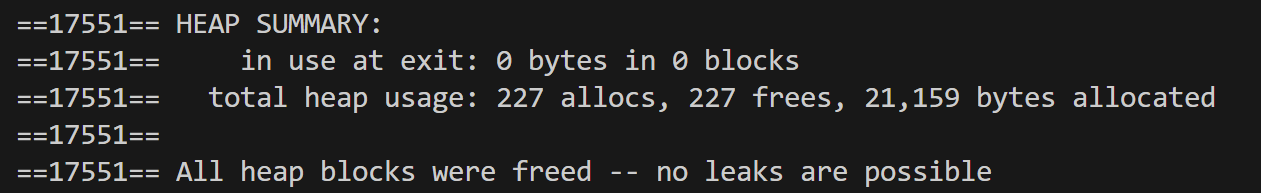
\includegraphics[width=0.6\textwidth]{valgrind.png}
    \caption{valgrind检测结果}
    \label{fig:valgrind}
\end{figure}

\section{补充}
我原本撰写了另一份的实现代码,参见\texttt{BST复杂分情况讨论版.h}的Line 210-452部分。
\begin{itemize}
    \item detachMin函数实际借用findMin函数,同时用寻亲操作进行善后。
    \item remove函数中分情况讨论,同时不用递归策略,利用自定义的find函数直接查找节点。
    \item 由于上述两种操作,因此无法直接用伴随递归的平衡操作。因此需要进行高度维护和回溯平衡。
    \item 因此,自己抽象了upgradeHeight的高度修改函数,目的是删除节点后,从根到树叶进行逐个高度修改。
    \item 以及回溯性的平衡函数retrospective\_balance,从树叶到根逐个进行平衡,回溯的过程调用自己集成的find\_parent寻亲函数,逐层向上。
    \item 在此基础上,在remove函数的实现中,对被删节点的各种情况分类讨论,并具体进行不同的高度维护、平衡操作。
\end{itemize}
但出现了复杂的段错误,且始终未能解决。应当还是分情况讨论的策略过于复杂,同时必须采用大量自定义的指针操作函数。
因此,一方面水平不足,同时时间有限,只能放弃这种实现策略。\\
全面覆写程序,在递归的同时自动进行高度的维护以及平衡操作,实现明显简单了很多。

\end{document}

